\documentclass[11pt]{article}

\usepackage[margin=1.15in]{geometry}
\usepackage{amsmath,amssymb,amsthm}
\usepackage{booktabs}
\usepackage{array}
\usepackage{enumitem}
\usepackage{microtype}
\usepackage{xcolor}
\usepackage{hyperref}
\usepackage{natbib}
\usepackage{titlesec}
\usepackage{multirow}
\usepackage{tikz}
\usetikzlibrary{positioning,fit,shapes.geometric,arrows.meta,calc,backgrounds,decorations.pathreplacing}

%% Figure colors
\definecolor{identity_c}{RGB}{180,120,50}
\definecolor{process_c}{RGB}{60,140,100}
\definecolor{math_c}{RGB}{60,100,180}
\definecolor{persp_c}{RGB}{160,80,160}
\definecolor{instru_c}{RGB}{150,60,60}
\definecolor{s0col}{RGB}{200,220,245}
\definecolor{s1col}{RGB}{190,235,200}
\definecolor{s2col}{RGB}{245,220,190}
\definecolor{s3col}{RGB}{220,200,235}
\definecolor{col1}{RGB}{70,130,180}
\definecolor{col2}{RGB}{180,100,60}
\definecolor{col3}{RGB}{80,150,100}
\definecolor{col4}{RGB}{140,90,160}
\definecolor{col5}{RGB}{160,130,60}
\definecolor{lightgrayfig}{RGB}{240,240,240}

\hypersetup{colorlinks=true,linkcolor=black,citecolor=black,urlcolor=blue}
\titleformat{\section}{\large\bfseries}{\thesection}{1em}{}
\titleformat{\subsection}{\normalsize\bfseries}{\thesubsection}{1em}{}

%% Theorem environments
\newtheorem{definition}{Definition}[section]
\newtheorem{proposition}{Proposition}[section]
\newtheorem{theorem}{Theorem}[section]
\newtheorem{conjecture}{Conjecture}[section]
\theoremstyle{remark}
\newtheorem{remark}{Remark}[section]
\newtheorem{example}{Example}[section]

%% Notation
\newcommand{\Gr}{\mathrm{Gr}}
\newcommand{\R}{\mathbb{R}}
\newcommand{\calM}{\mathcal{M}}
\newcommand{\calE}{\mathcal{E}}
\newcommand{\IIA}{\mathrm{IIA}}
\newcommand{\view}{\sigma}
\newcommand{\vO}{\mathcal{O}}
\newcommand{\vI}{\sim_{\sigma}}

\title{\textbf{What Is a Mechanism?}\\[0.3em]
\large An Atlas of Mechanistic Views for Interpretability Research}
\author{Elliot Tower\thanks{Working draft, June 2026. Companion to
  Tower (2026a) \emph{Mechanistic Validity} and Tower (2026b)
  \emph{The Geometry of Mechanisms}.}\\[0.2em]
\small Independent Researcher \quad \texttt{elliot@elliottower.ai}}
\date{Working draft, June 2026}

\begin{document}
\maketitle

\begin{abstract}
Mechanistic interpretability has produced circuits, features, causal
subspaces, and activation-steered algorithms.  Each result rests on an
implicit answer to a prior question: what kind of thing is a mechanism?
A head-level component, a functional role, a causal subspace, a
gauge-invariant structure, and a training-time trajectory carry
different identity criteria, require different evidence, and license
different inferences.  This is not a terminological inconvenience---it
means that many apparent disagreements in the literature are
ontological disagreements being argued at the wrong level.

This paper introduces \emph{mechanistic views}: explicit background
accounts of what mechanisms are, how they are identified, when two
descriptions refer to the same mechanism, and what evidence can
support claims about them.  A view is a tuple $(O, {\sim}, E, F, T)$
where $O$ is a set of mechanism candidates, ${\sim}$ is an equivalence
relation on $O$ specifying identity, $E$ is an evidential standard, $F$
is the appropriate formalism, and $T$ is the explanatory target.  We
state coherence conditions on the tuple and prove that incoherent views
produce systematically unsatisfiable evidential demands.

We organize the space of possible views along five axes and present an
atlas of eight views currently operative in the interpretability
literature: object, role, subspace, structural, process, stratified,
perspectival, and instrumental.  For each view we give the full axis
assignments, characteristic evidence types, failure modes, and the
experiments that would discriminate it from neighboring views.  We show
that the axes are not independent: ontology determines identity
determines formalism, a chain that explains why most coherence violations
are mismatches between the first three axes.  A five-axis methods mapping
classifies 15 common interpretability tools by their implicit view
commitments, revealing that most methods are Object view with activation
evidence, and identifying DAS as a Role-view method with borrowed
subspace parameterization.  We then develop three worked examples at
depth---IOI, induction heads, and SAE features---showing what each view
claims, what it licenses, and what evidence remains open.  Finally, we
identify five recurring decision points in empirical work and explain
what each view implies for them.

The framework is not a proposal for a single correct ontology.  It is a
diagnostic tool: making the view explicit lets researchers state claims
at the level their evidence supports, locate disagreements at their
source, and design experiments that discriminate views rather than
confirming them.
\end{abstract}

\tableofcontents
\newpage

%% ---------------------------------------------------------------
\section{Introduction}
%% ---------------------------------------------------------------

Mechanistic interpretability aims to explain what trained neural
networks are computing.  The field has made this aim concrete:
transformer circuits provide a component-level vocabulary for attention
heads and MLPs \citep{elhage2021}; induction heads account for a
mechanism involved in in-context learning \citep{olsson2022}; the
indirect object identification (IOI) circuit names the attention heads
involved in a specific syntactic task \citep{wang2022}; sparse
autoencoders recover interpretable directions from activation spaces
\citep{bricken2023,templeton2024}; causal abstraction methods test
whether high-level variables are realized in distributed representations
\citep{geiger2021,geiger2024}; and weight-space analyses recover circuit
structure without forward passes \citep{tower2026weight}.

Yet the word \emph{mechanism} does not mean the same thing in all of
these cases.  In one paper a mechanism is a set of attention heads;
in another it is a functional role such as ``name mover''; in another
it is a causal subspace recovered by distributed alignment search; in
another it is a training-time transition.  These are not merely
terminological differences.  They carry different answers to five basic
questions:
\begin{enumerate}[leftmargin=*,label=(\arabic*)]
\item \textbf{Ontology}: what kind of entity counts as a mechanism?
\item \textbf{Identity}: when do two descriptions refer to the same mechanism?
\item \textbf{Evidence}: what measurements can warrant a claim about a mechanism?
\item \textbf{Formalism}: what mathematical language expresses the claim?
\item \textbf{Target}: what phenomenon is the mechanism supposed to explain?
\end{enumerate}
Most published work answers these questions implicitly.  The answers are
recoverable from the methods used and the conclusions drawn, but they are
not stated---and because they are not stated, disagreements that are
fundamentally ontological are argued as disagreements about experimental
design.

\paragraph{Three motivating cases.}

\textbf{Underdetermination.}  Activation patching establishes that a
head is causally relevant to a behavior.  Does this establish a
mechanism?  Under the object view, perhaps yes.  Under the role view,
only if the functional role is independently specified and tested.
Under the subspace view, not unless the relevant variable is localized
to a specific causal subspace.  Under the structural view, not unless
the result is invariant under the relevant parameter symmetries.  A
single activation-patching result means different things under different
views, and the disagreement cannot be resolved by further patching
experiments alone---because all such experiments are equally consistent
with multiple views.

\textbf{Cross-model comparison.}  The claim that GPT-2 Small and
Pythia-160M implement the same induction head mechanism requires a
notion of mechanism identity that is cross-model.  Component indices are
trivially not cross-model.  Functional roles may be, if independently
specified.  Gauge-invariant subspace structure may be, if a canonical
transport map is defined.  Training-time trajectories may be, if the
dynamical basins correspond.  Which notion is operative determines
whether ``the same mechanism'' is meaningful across architectures---and
therefore whether cross-model generalization claims are well-formed.

\textbf{Safety-relevant inference.}  Safety work reasons from ``circuit
$X$ is present'' to ``the model has goal $Y$'' or ``the model would
behave $Z$ under distribution shift.''  These inferences require
different things depending on what a mechanism is.  Under an object view,
circuit presence is a fact about specific components in a specific model
on a specific distribution.  Under a structural view, a circuit present
as a gauge-invariant structure is robust to reparameterization.  Under
the instrumental view, a circuit label is warranted by behavioral
predictions.  The inference from circuit presence to safety-relevant
conclusion requires specifying which of these is operative.

\paragraph{Contributions.}
This paper makes the following contributions:
\begin{enumerate}[leftmargin=*]
\item A formal definition of a \emph{mechanistic view} as a five-component
      structure $(O, {\sim}, E, F, T)$ with typed components and coherence
      conditions stated as propositions (\S\ref{sec:views}).
\item An atlas of eight views currently operative in the
      interpretability literature, with full axis assignments, evidence
      standards, discriminating experiments, and failure modes
      (\S\ref{sec:atlas}).
\item The determination chain: ontology implies identity implies formalism,
      with a five-axis methods mapping showing how common tools carry
      implicit view commitments (\S\ref{sec:chain}, \S\ref{sec:methods}).
\item Three worked examples---IOI, induction heads, SAE features---showing
      what each view claims, what it licenses, and what evidence is needed
      to advance from one view to another (\S\ref{sec:examples}).
\item An analysis of five recurring decision points in empirical work and
      what each view implies for them (\S\ref{sec:decisions}).
\item Positioning of Mechanistic Views relative to the companion
      frameworks of Mechanistic Validity \citep{tower2026mechval} and the
      Geometry of Mechanisms \citep{tower2026geom}, with explicit
      identification of what each framework presupposes and what it provides
      (\S\ref{sec:companions}).
\end{enumerate}

\paragraph{What this paper is not.}
It is not a proposal to replace the eight views with a single preferred
ontology.  Each view is appropriate for some questions and inappropriate
for others.  The goal is to make view choice explicit so that it can be
justified or revised, not to eliminate plurality.  It is also not a
paper about methodology per se: methods (patching, DAS, SAEs,
weight-space analysis) are discussed only in their relation to views,
not evaluated on their own technical merits.

\paragraph{Relationship to companion papers.}
MechVal \citep{tower2026mechval} provides criteria for evaluating
whether a mechanistic claim is warranted by evidence.  Those criteria
presuppose that the claim type is fixed.  The Geometry of Mechanisms
\citep{tower2026geom} provides the formal mathematical objects---Grassmannian
structural causal models, parallel transport, holonomy, sheaf
cohomology---that the subspace and structural views implicitly require.
That formalism presupposes that the subspace view is appropriate.  The
present paper asks what makes those presuppositions explicit and
justifiable.

%% ---------------------------------------------------------------
\section{Mechanistic Views}\label{sec:views}
%% ---------------------------------------------------------------

\subsection{Formal Definition}

A mechanistic view is a background commitment that a researcher makes,
explicitly or implicitly, when they ask what a mechanism is.  We give
a formal definition, then unpack each component.

\begin{definition}[Mechanistic view]\label{def:view}
A \emph{mechanistic view} $\view$ is a tuple $(O, {\sim}, E, F, T)$
where:
\begin{enumerate}[leftmargin=*, label=(\roman*)]
\item $O$ is a set, the \textbf{ontology}, whose elements are the
      entities that count as mechanisms under $\view$.
\item ${\sim} \subseteq O \times O$ is an equivalence relation on $O$,
      the \textbf{identity criterion}: $x \sim y$ means descriptions $x$
      and $y$ refer to the same mechanism under $\view$.
\item $E$ is a set of \textbf{evidential standards}: pairs
      $(m, C)$ where $m$ is a measurement type and $C \subseteq
      2^O/{\sim}$ is the set of claims about equivalence classes of
      mechanisms that $m$ can in principle support.
\item $F$ is a \textbf{formalism}: a mathematical or representational
      language in which elements of $O$ can be expressed and $\sim$ can
      be computed.
\item $T$ is a \textbf{target}: a specification of the phenomena the
      view is designed to explain.
\end{enumerate}
\end{definition}

Several features of Definition~\ref{def:view} deserve comment.

The identity criterion $\sim$ is required to be an equivalence relation
(reflexive, symmetric, transitive).  This is not automatic: some
informal notions of mechanism identity in the literature are not
transitive.  For example, saying mechanisms $A$ and $B$ are ``related''
by shared components, and $B$ and $C$ are ``related'' by shared
function, does not imply $A$ and $C$ are the same mechanism.  Making
$\sim$ an equivalence relation forces precision.

The evidential standard $E$ is explicitly typed: each measurement type
$m$ is associated with the claims $C$ it can support.  This rules out
the common practice of using a measurement to support a claim that is
not in the range of that measurement.  Activation patching establishes
causal relevance of a component; it is not in the range of subspace
localization claims unless supplemented.

\begin{definition}[Coherence]\label{def:coherence}
A view $\view = (O, {\sim}, E, F, T)$ is \emph{coherent} if:
\begin{enumerate}[leftmargin=*, label=(\roman*)]
\item \textbf{Identity is grounded}: $\sim$ is definable using only
      the objects in $O$ and the language of $F$.  (A view whose
      identity criterion involves objects not in its own ontology is
      incoherent.)
\item \textbf{Evidence tracks identity}: for every measurement type
      $m \in E$, the claims $C(m)$ are expressible in terms of $\sim$-classes,
      not finer-grained distinctions.  (Evidence that distinguishes objects
      within a $\sim$-class is picking up on a different ontology than
      the one declared.)
\item \textbf{Formalism is expressive}: every element of $O$ has a
      representation in $F$, and $\sim$ is computable in $F$.
\end{enumerate}
\end{definition}

\begin{proposition}[Incoherent views produce contradictory demands]\label{prop:incoherence}
Let $\view = (O, {\sim}, E, F, T)$ be a view that violates coherence
condition (ii): there exists a measurement type $m \in E$ and objects
$x, y \in O$ with $x \sim y$ but $m(x) \neq m(y)$.  Then there exist
mechanistic claims that are simultaneously required by $\sim$ to be true
(since $x$ and $y$ are the same mechanism) and required by $E$ to be
false (since $m$ distinguishes them).  No experiment can satisfy both
demands.
\end{proposition}

\begin{proof}
Let $\phi$ be the claim ``$x$ and $y$ are the same mechanism.''  Since
$x \sim y$, $\phi$ is true under $\view$.  The measurement $m$ produces
$m(x) \neq m(y)$.  If $m$ is an evidence type for mechanism identity
(i.e., different $m$-values imply different mechanisms), then $m(x) \neq
m(y)$ implies $\phi$ is false.  The view asserts $\phi$ and $\neg \phi$
simultaneously.  \hfill $\square$
\end{proof}

Proposition~\ref{prop:incoherence} is useful diagnostically.  A common
pattern in interpretability is to declare that mechanisms are
gauge-invariant structures (structural view ontology) but then to use
activation-patching results as evidence of mechanism presence without
checking gauge invariance.  If the patching result changes under a
reparameterization that preserves computation, it is distinguishing
objects that the structural view says are identical.

\subsection{The Five Axes}\label{sec:axes}

We organize the components of Definition~\ref{def:view} into five named
axes.  The axes are not independent: as coherence requires, choices on
one axis constrain the others.

\paragraph{Ontology ($O$).}
What kind of entity counts as a mechanism?  Options include: concrete
model components (heads, neurons, MLP sublayers, SAE dictionary
elements), functional roles (descriptions of what a component does
independently of which component does it), causal subspaces (linear or
nonlinear submanifolds of the residual stream that mediate a causal
variable), gauge-invariant structures (equivalence classes of weight
configurations under symmetries that preserve the computation),
temporally extended processes (formation pathways or execution
trajectories), points in a stratified mechanism space, measurement
perspectives, and predictive models.

\paragraph{Identity ($\sim$).}
When do two mechanism descriptions denote the same mechanism?  Options
include: component overlap ($x \sim y$ iff they name the same set of
heads or neurons), role equivalence ($x \sim y$ iff they specify the
same functional input--output mapping), subspace proximity ($x \sim y$
iff the principal angles between the causal subspaces are all below a
threshold $\theta$, i.e.\ geodesic distance on $\Gr(k,d)$ is small),
gauge-orbit membership ($x \sim y$ iff there exists a computation-preserving
symmetry $g$ with $g \cdot x = y$), and dynamical-basin membership
($x \sim y$ iff the formation trajectories converge to the same
attractor).

\paragraph{Evidence ($E$).}
What measurements can support what claims?  Key distinctions: activation
patching establishes causal relevance of components under a fixed
distribution; DAS/IIA with linear alignment constraints measures causal
subspace identity; weight composition scores measure structural
information flow independent of any input distribution; checkpoint
analysis establishes formation dynamics; multi-method robustness tests
perspectival convergence.

\paragraph{Formalism ($F$).}
What representational language is appropriate?  Directed graphs (circuits);
functional decompositions (roles); Grassmannian geometry $\Gr(k,d)$
(subspaces); fiber bundles and gauge groups (structural view); dynamical
systems and phase portraits (process view); Whitney stratifications
(stratified view); measurement algebras (perspectival view).

\paragraph{Target ($T$).}
What is the mechanism supposed to explain?  A specific behavioral output
on a specific distribution; a functional class across models; a
representational variable across inputs; a computation class across
parameterizations; a formation event; a resolution-relative phenomenon;
or a behavioral prediction.

%% ---------------------------------------------------------------
\section{An Atlas of Views}\label{sec:atlas}
%% ---------------------------------------------------------------

We identify eight views currently operative in the literature.  Table~\ref{tab:atlas}
gives the full axis assignments; Figure~\ref{fig:axes} shows how the five axes organize
the eight views.  The views are not mutually exclusive:
a single paper may use several, and convergence across views constitutes
stronger evidence than any single view.  The point is to distinguish
them so that each view's commitments and limitations can be assessed
independently.

\begin{table}[ht]
\centering
\small
\setlength{\tabcolsep}{4pt}
\begin{tabular}{p{0.10\linewidth}p{0.15\linewidth}p{0.15\linewidth}p{0.17\linewidth}p{0.15\linewidth}p{0.15\linewidth}}
\toprule
\textbf{View} & \textbf{Ontology ($O$)} & \textbf{Identity ($\sim$)}
  & \textbf{Evidence ($E$)} & \textbf{Formalism ($F$)} & \textbf{Target ($T$)} \\
\midrule
Object
  & Concrete part: head, neuron, feature
  & Component overlap
  & Ablation, activation patching
  & Directed graph
  & Specific behavior \\[3pt]
Role
  & Functional role in computation
  & Role equivalence (same I/O mapping)
  & Role-specific causal tests, cross-model
  & Functional decomposition
  & Functional class \\[3pt]
Subspace
  & Causal subspace of residual stream
  & Same projector; $d_{\Gr} < \theta$
  & DAS/IIA (linear), subspace stability
  & $\Gr(k,d)$
  & Representational variable \\[3pt]
Structural
  & Gauge-invariant relational structure
  & Gauge-orbit membership
  & Holonomy, comp. scores, reparameterization
  & Fiber bundle quotient
  & Computation class \\[3pt]
Process
  & Formation trajectory or execution regime
  & Same trajectory type or dynamical basin
  & Training checkpoints, formation knockouts
  & Dynamical system
  & Mechanism origin \\[3pt]
Stratified
  & Point in stratified mechanism space
  & Same stratum + local equivalence
  & Dimensionality tests, localization diagnostics
  & Whitney stratification
  & Resolution-relative phenomenon \\[3pt]
Perspectival
  & Projection of mechanism onto context
  & Cross-method coherence
  & Multi-method robustness
  & Measurement algebra
  & Method-relative observation \\[3pt]
Instrumental
  & Useful predictive or interventional model
  & Predictive equivalence
  & Forecast accuracy, intervention utility
  & Model theory
  & Behavioral prediction \\
\bottomrule
\end{tabular}
\caption{The eight mechanistic views with full axis assignments.}
\label{tab:atlas}
\end{table}


\begin{figure}[t]
\centering
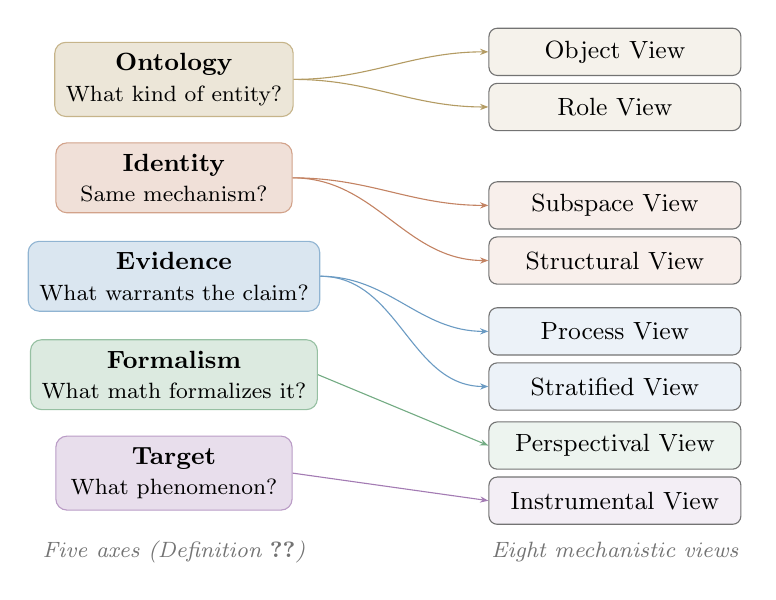
\begin{tikzpicture}[
  every node/.style={font=\small},
  axis/.style={draw=black!60, fill=lightgrayfig, rounded corners=4pt,
               minimum width=3.0cm, minimum height=0.65cm, align=center, inner sep=4pt},
  view/.style={draw=black!55, rounded corners=3pt,
               minimum width=3.2cm, minimum height=0.6cm, align=center, inner sep=3pt},
  arr/.style={-{Stealth[length=3pt]}, thin},
]
\node[axis, fill=col5!20, draw=col5!60] (ax1) at (0,0)     {\textbf{Ontology}\\{\footnotesize What kind of entity?}};
\node[axis, fill=col2!20, draw=col2!60] (ax2) at (0,-1.25) {\textbf{Identity}\\{\footnotesize Same mechanism?}};
\node[axis, fill=col1!20, draw=col1!60] (ax3) at (0,-2.5)  {\textbf{Evidence}\\{\footnotesize What warrants the claim?}};
\node[axis, fill=col3!20, draw=col3!60] (ax4) at (0,-3.75) {\textbf{Formalism}\\{\footnotesize What math formalizes it?}};
\node[axis, fill=col4!20, draw=col4!60] (ax5) at (0,-5.0)  {\textbf{Target}\\{\footnotesize What phenomenon?}};
\node[view, fill=col5!10] (v_obj)   at (5.6, 0.35)  {Object View};
\node[view, fill=col5!10] (v_rol)   at (5.6,-0.35)  {Role View};
\node[view, fill=col2!10] (v_sub)   at (5.6,-1.6)   {Subspace View};
\node[view, fill=col2!10] (v_str)   at (5.6,-2.3)   {Structural View};
\node[view, fill=col1!10] (v_pro)   at (5.6,-3.2)   {Process View};
\node[view, fill=col1!10] (v_strat) at (5.6,-3.9)   {Stratified View};
\node[view, fill=col3!10] (v_per)   at (5.6,-4.65)  {Perspectival View};
\node[view, fill=col4!10] (v_ins)   at (5.6,-5.35)  {Instrumental View};
\draw[arr, col5!80] (ax1.east) to[out=0,in=180] (v_obj.west);
\draw[arr, col5!80] (ax1.east) to[out=0,in=180] (v_rol.west);
\draw[arr, col2!80] (ax2.east) to[out=0,in=180] (v_sub.west);
\draw[arr, col2!80] (ax2.east) to[out=0,in=180] (v_str.west);
\draw[arr, col1!80] (ax3.east) to[out=0,in=180] (v_pro.west);
\draw[arr, col1!80] (ax3.east) to[out=0,in=180] (v_strat.west);
\draw[arr, col3!80] (ax4.east) -- (v_per.west);
\draw[arr, col4!80] (ax5.east) -- (v_ins.west);
\node[font=\footnotesize\itshape, text=black!55] at (0,-6.0) {Five axes (Definition~\ref{def:view})};
\node[font=\footnotesize\itshape, text=black!55] at (5.6,-6.0) {Eight mechanistic views};
\end{tikzpicture}
\caption{The five axes of a mechanistic view (left) correspond to the five components
  of Definition~\ref{def:view}: $(O, {\sim}, E, F, T)$.  Each axis maps to one or
  more of the eight views (right).  The mapping is not one-to-one: the ontology axis
  distinguishes the object and role views by their commitment level; the identity axis
  distinguishes the subspace and structural views by whether identity is geometric
  or gauge-theoretic.}
\label{fig:axes}
\end{figure}

\subsection{Object View}

The object view treats mechanisms as concrete model components: specific
attention heads, neurons, MLP sublayers, or sparse autoencoder dictionary
elements.  It is the implicit view in circuit diagrams.  The IOI circuit
as reported by \citet{wang2022}---26 attention heads organized into
functional groups---is an object-level description: the claim is about
those specific computational units.

\paragraph{Identity.}
Two circuit descriptions refer to the same mechanism iff they name the
same components.  This is precise within a model but trivially fails
cross-model: a head in GPT-2 Small is not an object in Pythia-160M.

\paragraph{Evidence.}
Ablation and activation patching are the natural evidence types.  Removing
a component's activation and observing behavioral degradation establishes
causal necessity; replacing it with a counterfactual activation establishes
causal sufficiency relative to that counterfactual.  The method is
strongest when the component set is stable across prompt distributions
and the ablation effect is large and specific.

\paragraph{Failure modes.}
\emph{Role inflation}: a component is identified by patching, then labeled
with a role (``name mover,'' ``induction head'') that implies richer
mechanistic content than the object-level evidence supports.  The component
identity is established; the role is a hypothesis.  \emph{Distribution
sensitivity}: the circuit identified by patching on one distribution may
differ substantially on another, meaning the claimed object-level mechanism
is distribution-relative.

\paragraph{Discriminating experiment.}
To test whether the object view is appropriate: ablate the identified
component set and test whether behavioral degradation is (a)~specific to
the behavior the mechanism is supposed to implement and (b)~stable across
prompt distributions.  If (b) fails, the object-level description is
distribution-relative and a role or subspace description may be more
appropriate.

\subsection{Role View}

The role view treats mechanisms as functional roles that can be realized
by different components.  ``Name mover'' is a role: it describes what a
component does (copy a name token to the output position), not which head
does it.  The role view explains why functionally equivalent components
across different models can be meaningfully compared.

\paragraph{Identity.}
Same functional input--output role, possibly in different components or
models.  Role identity requires a specification of the role that is
independent of the discovery procedure (i.e., not merely ``does what
this head does'') and tests that go beyond the ablation that revealed
the component.

\paragraph{Evidence.}
Role-specific predictions that are not entailed by mere causal relevance.
For a name-mover role claim: the weight-space signature of $W_{OV}$
should encode a copying operation; the head should perform this function
on novel prompts; a head in a different model with the same $W_{OV}$
signature should earn the same label.  \citet{tower2026mechval} identifies
the object-to-role slide as a common source of overclaiming: establishing
that head 9.9 is causally necessary for IOI does not establish that it
is a name mover until the role is independently operationalized and tested.

\paragraph{Failure modes.}
\emph{Role proliferation}: a new role label is coined for each component
discovered, re-describing the data without adding explanatory content.
\emph{Underdefined roles}: role labels are informal enough to be true of
any component, making them unfalsifiable.

\paragraph{Discriminating experiment.}
Take the role specification and apply it to a model in which the
original component has been ablated.  If the role is real, either another
component should take over (backup mechanism) or the behavior should
degrade in a specific role-consistent way.  If no such prediction is
confirmed, the role label has not been independently validated.

\subsection{Subspace View}

The subspace view treats mechanisms as low-dimensional causal subspaces
of the residual stream.  The key observation is that distributed
alignment search \citep{geiger2021,geiger2024} identifies not a component
but a rotation of the activation space: the causal variable is encoded
in a subspace that may span many components.  If alignment matrix $Q$
and its rotation $QR$ both achieve the same interchange intervention
accuracy (IIA), the relevant object is the subspace $\mathrm{span}(Q)$,
not the matrix $Q$.

\paragraph{Identity.}
Two subspace mechanisms are the same iff they project onto the same
subspace of $\mathbb{R}^d$: same projector $QQ^\top$, or equivalently
small geodesic distance on $\Gr(k,d)$.  This is basis-invariant and
can be meaningful cross-model when corresponding residual streams can
be aligned.

\paragraph{Evidence.}
DAS and IIA, subject to a critical constraint.  \citet{sutter2025}
showed that unrestricted nonlinear alignment maps achieve $100\%$ IIA
even on randomly initialized models, making DAS vacuous without
structural constraints on the alignment class.  Subspace-view claims
therefore require either linear alignment or alignment constrained to
respect the transport structure induced by the weight matrices.  Subject
to this constraint, subspace stability (eigenvalue gap between the causal
subspace and its complement) is the natural diagnostic.

\paragraph{Failure modes.}
\emph{SAE confusion}: sparse autoencoder features are dictionary elements
that minimize reconstruction loss; causal subspaces are directions that
mediate specific causal paths.  These are different objectives and can
disagree.  An SAE feature is a hypothesis about a one-dimensional
subspace mechanism, not a confirmed subspace claim.  \emph{Sutter vacuousness}:
reporting high IIA without specifying the alignment class allows any
model to be assigned any causal structure.

\paragraph{Discriminating experiment.}
Verify that the identified subspace is stable: the subspace recovered
by DAS on a held-out distribution should have small geodesic distance
from the training-distribution subspace.  Also confirm that
an aligned basis-change (within the subspace) does not change the IIA,
while a rotation that takes vectors out of the subspace does reduce it.

\subsection{Structural View}

The structural view treats mechanisms as equivalence classes of
implementations under transformations that preserve the computation.
The relevant object is not a head index, a basis vector, or a specific
projection---it is the orbit of implementations related by the symmetry
group of the transformer's weight space.  Two weight configurations
that implement the same computation via different parameterizations are
the same mechanism under this view.

The formalism involves gauge orbits, parallel transport maps on the
Grassmannian, holonomy groups, and sheaf cohomology, developed in
\citet{tower2026geom}.

\paragraph{Identity.}
Gauge-orbit membership: $x \sim y$ iff there exists a computation-preserving
symmetry $g$ (such as a scale transformation, a rotation of a head's
query-key subspace paired with an inverse rotation of its output, or a
permutation of neurons) such that $g \cdot x = y$.  Holonomy fingerprints
provide a finer criterion: the holonomy group of the transport map
induced by a mechanism's weight matrices is an invariant that does not
change under gauge transformations.

\paragraph{Evidence.}
Gauge-invariant measurements: weight-space composition scores
$\|W_{O,u} W_{K,v}\|_F$ measure information flow capacity independently
of basis choice \citep{tower2026weight}; holonomy measurements; and
reparameterization-stability tests (check that a result survives
computation-preserving rescalings of the weights).

\paragraph{Failure modes.}
\emph{False gauge invariance}: claiming structural equivalence without
verifying that the symmetry actually preserves the computation.
\emph{Architectural prior confound}: structural features that
discriminate trained from randomly initialized models may be detecting
architecturally privileged positions rather than learned structure
\citep{tower2026weight}.

\paragraph{Discriminating experiment.}
Apply a known computation-preserving symmetry (e.g., scale by $\lambda$,
counter-scale by $\lambda^{-1}$) to the weights of a component and
retest the activation-space evidence.  If the activation-space result
changes, the original result was not gauge-invariant and is not a
structural-view claim.

\subsection{Process View}

The process view treats mechanisms as temporally extended.  A mechanism
is not merely a final-checkpoint artifact but a formation process, an
execution trajectory, or a dynamical regime.  This view is natural for
phenomena where the how of learning is itself mechanistically relevant:
the induction head mechanism, for instance, forms via a phase transition
at a specific training step \citep{olsson2022}---this is process-level
structure that is not recoverable from the final checkpoint alone.

\paragraph{Identity.}
Same trajectory type or dynamical basin.  Two processes are the same
mechanism if they follow the same formation pathway, occupy the same
attractor, or exhibit the same phase-transition structure.  This notion
of identity is less developed than component or subspace identity, and
formalizing it is an open problem.

\paragraph{Evidence.}
Checkpoints, gradient flow, loss-curve structure, and formation knockouts.
A mechanism claim under the process view cannot be supported by
final-checkpoint analysis alone.  The induction head formation result
provides a clear example: the phase change at a specific training step
is visible in the composition score evolution, and this is process-level
evidence distinct from any claim about the final circuit \citep{olsson2022}.

\paragraph{Failure modes.}
\emph{Process--circuit conflation}: the final-checkpoint circuit and the
formation process are distinct objects; the circuit does not determine
the process.  Two models may arrive at identical final circuits via very
different training trajectories.  \emph{Training-detail overfitting}: a
process described precisely enough to be informative may be specific to
a particular optimizer, learning rate schedule, or dataset.

\paragraph{Discriminating experiment.}
Run the same architecture with different training hyperparameters (learning
rate, batch size, optimizer) and compare the formation dynamics.  If the
final circuit is similar but the formation trajectory differs, the
process-level claim is hyperparameter-sensitive and should be stated at
the appropriate level of generality.

\subsection{Stratified View}

The stratified view treats mechanism space as organized into strata:
point-localized objects, one-dimensional features, higher-dimensional
subspaces, nonlinear manifolds, and fully distributed structures.  Rather
than forcing a binary choice between localized and distributed, the
stratified view asks which stratum the evidence supports and whether the
appropriate description changes with measurement resolution.


\begin{figure}[t]
\centering
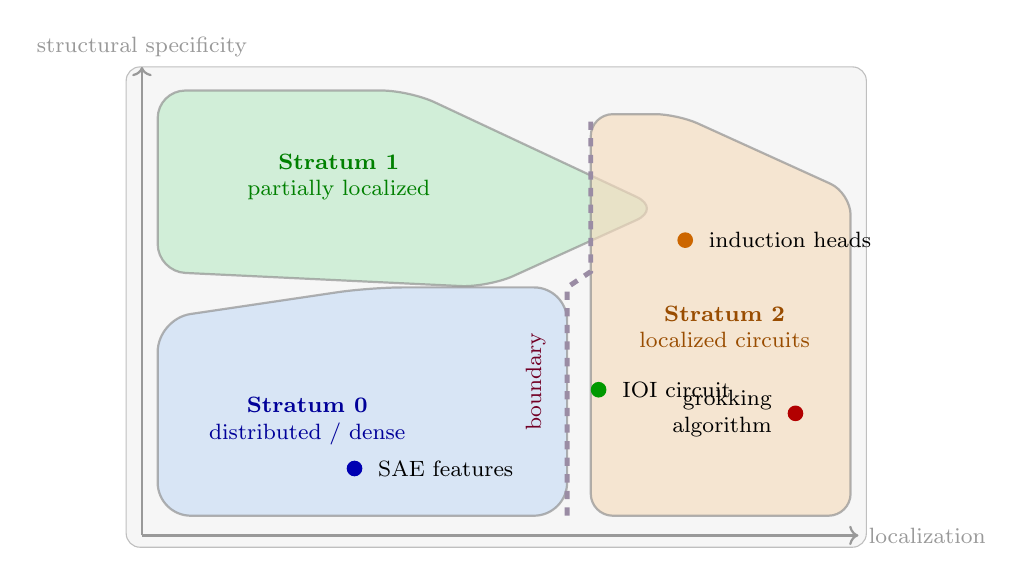
\begin{tikzpicture}[
  every node/.style={font=\small},
  stratum/.style={draw=black!45, line width=0.8pt},
  pt/.style={circle, fill, inner sep=2.0pt},
  lab/.style={font=\footnotesize, align=center},
]
\fill[gray!7, draw=black!25, rounded corners=5pt] (-0.3,-0.3) rectangle (9.1,5.8);
\fill[s0col, opacity=0.65, stratum, rounded corners=12pt]
  (0.1,0.1) -- (5.3,0.1) -- (5.3,3.0) -- (2.8,3.0) -- (0.1,2.6) -- cycle;
\node[lab, text=blue!60!black] at (2.0,1.3) {\textbf{Stratum~0}\\distributed / dense};
\fill[s1col, opacity=0.65, stratum, rounded corners=10pt]
  (0.1,3.2) -- (4.3,3.0) -- (6.5,4.0) -- (3.3,5.5) -- (0.1,5.5) -- cycle;
\node[lab, text=green!50!black] at (2.4,4.4) {\textbf{Stratum~1}\\partially localized};
\fill[s2col, opacity=0.65, stratum, rounded corners=8pt]
  (5.6,0.1) -- (8.9,0.1) -- (8.9,4.2) -- (6.7,5.2) -- (5.6,5.2) -- (5.6,3.2) -- cycle;
\node[lab, text=orange!60!black] at (7.3,2.5) {\textbf{Stratum~2}\\localized circuits};
\draw[s3col!70!black, line width=1.8pt, dashed]
  (5.3,0.1) -- (5.3,3.0) -- (5.6,3.2) -- (5.6,5.2);
\node[lab, text=purple!60!black, rotate=90] at (4.9,1.8) {\footnotesize boundary};
\node[pt, fill=orange!80!black] (ih)   at (6.8,3.6) {};
\node[right=2pt of ih,  lab, align=left] {\footnotesize induction heads};
\node[pt, fill=green!60!black]  (ioi)  at (5.7,1.7) {};
\node[right=2pt of ioi, lab, align=left] {\footnotesize IOI circuit};
\node[pt, fill=blue!70!black]   (sae)  at (2.6,0.7) {};
\node[right=2pt of sae, lab, align=left] {\footnotesize SAE features};
\node[pt, fill=red!70!black]    (grok) at (8.2,1.4) {};
\node[left=2pt  of grok, lab, align=right] {\footnotesize grokking\\ algorithm};
\draw[->, black!40, thick] (-0.1,-0.15) -- (9.0,-0.15) node[right, font=\footnotesize] {localization};
\draw[->, black!40, thick] (-0.1,-0.15) -- (-0.1,5.8)  node[above, font=\footnotesize] {structural specificity};
\end{tikzpicture}
\caption{Schematic of mechanism space as a stratified manifold.  Each stratum
  is a smoothly varying subset distinguished by the localization and structural
  specificity of the mechanism.  Boundaries between strata are lower-dimensional
  singular sets.  Empirical examples are placed roughly by the evidence reviewed
  in Section~\ref{sec:examples}; exact positions are schematic, not quantitative.}
\label{fig:strata}
\end{figure}

Figure~\ref{fig:strata} illustrates the key distinctions schematically.
The natural formalism is Whitney stratification: a decomposition of
mechanism space into smooth manifold strata that are partially ordered
by containment of their closures.  A mechanism's stratum is determined
by its dimensionality, its localizability in specific components, and
the topology of its support in the residual stream.

\paragraph{Identity.}
Same stratum and same local equivalence class within the stratum.  Two
descriptions are the same mechanism if they name the same stratum and
agree on local structure within that stratum.

\paragraph{Evidence.}
Dimensionality tests (effective rank of the causal subspace),
localization diagnostics (is the mechanism's effect concentrated in a
small component set or distributed?), and stratum-transition tests
(does the apparent mechanism change stratum when the measurement
resolution changes?).

\paragraph{Failure modes.}
\emph{Stratum misidentification from method artifacts.}  A genuinely
distributed mechanism may appear localized to a single component if
the ablation method captures only the dominant direction.  Conversely,
a localized mechanism may appear distributed if the measurement method
has high background noise.  The stratified view does not resolve this
automatically---it provides the language to state it precisely.

\paragraph{Discriminating experiment.}
The stratified view predicts that measurement resolution affects the
apparent stratum.  Test this by comparing the effective dimensionality
of the causal subspace recovered by DAS at different hook points and
with different alignment constraints.  Consistent stratum across
resolutions supports a stratum assignment; stratum-change suggests
either a higher-stratum mechanism being partially recovered or a
measurement artifact.

\subsection{Perspectival View}

The perspectival view treats methods as revealing partial projections of
mechanisms rather than the mechanism in itself.  Activation patching,
weight analysis, DAS, and sparse autoencoders are different perspectives
with different invariances and different blind spots.  Disagreement
between methods is therefore not automatically a failure; it may reveal
the method-relative structure of what is being measured.

This view is philosophically related to Massimi's perspectival realism
\citep{massimi2022}: the claim is not that mechanisms are relative to
methods (that would be instrumentalism), but that scientific methods
are partial perspectives on a method-independent mechanistic structure.
Mechanistic claims are not merely predictions---they have a realist
reading---but each method can only support claims about the aspect of
the mechanism it is sensitive to.

\paragraph{Identity.}
Coherence across perspectives.  Two descriptions refer to the same
mechanism if they are mutually consistent and jointly interpretable as
projections of the same underlying structure.  This is weaker than
convergence (the descriptions need not agree quantitatively) but
stronger than mere non-contradiction.

\paragraph{Evidence.}
Multi-method robustness.  A mechanistic claim supported by a single
method is vulnerable to that method's specific confounds; a claim
supported by convergent evidence from methods with different
assumptions is stronger.  MechVal \citep{tower2026mechval} formalizes
this as a convergence requirement across three evidence families:
structural (weight), causal (activation/intervention), and dynamic
(training-time).

\paragraph{Failure modes.}
\emph{Perspectival conflation}: treating a method-specific disagreement
as evidence against the existence of the mechanism, rather than as
information about which aspect each method is tracking.
\emph{Anti-realist slide}: treating the method-relativity of evidence
as implying that mechanisms are method-relative objects---conflating the
perspectivality of evidence with the perspectivality of truth.

\paragraph{Discriminating experiment.}
Take a mechanistic claim supported by patching and test whether the
weight-space composition score for the same component is consistent
with the claimed causal role.  If the weight-space result is inconsistent,
this is either a perspectival disagreement (the two methods track
different aspects of the structure) or a failure of one method.
Adjudicating which requires a third method.

\subsection{Instrumental View}

The instrumental view treats mechanisms as useful predictive or
interventional models.  On this view, a mechanism claim is warranted if
it helps predict or control the model, regardless of whether it
identifies a real internal object.  The label ``head 9.9 is a name
mover'' is warranted if it generates accurate behavioral predictions
and effective interventions, not because the head has an intrinsic
name-moving property.

\paragraph{Identity.}
Predictive equivalence.  Two descriptions are the same mechanism if
they make the same predictions about all interventions and all relevant
behaviors.  This is behaviorism at the level of mechanism descriptions.

\paragraph{Evidence.}
Forecast accuracy and intervention utility.  A mechanism label is
justified to the extent that novel behaviors predicted from it are
confirmed and interventions derived from it have the expected effects.

\paragraph{Failure modes.}
The instrumental view has the weakest ontological commitments and is
therefore the easiest to satisfy---but this is also its primary
limitation.  \emph{Safety-relevant overreach}: claims that require
strong ontological conclusions (``the model is pursuing a goal'',
``this behavior would persist under distribution shift'') cannot be
supported by predictive utility on the training distribution alone.
A mechanism that predicts behavior on seen distributions may fail
on unseen ones in ways that an object- or structure-level account
would anticipate.

\paragraph{Discriminating experiment.}
Test whether the mechanism label generates predictions that go beyond
the behavior used to identify it.  If a head is labeled a name mover,
it should predict name-moving behavior in novel syntactic constructions
not present in the original test suite.  Failure of novel prediction
at the same rate as success on the original test is evidence for an
overfitted label.

\subsection{The Determination Chain: Ontology Implies Identity Implies Formalism}\label{sec:chain}

The five axes are not independent.  In practice, the relationship is
mostly a chain of determination:
\[
\text{Ontology} \;\longrightarrow\; \text{Identity} \;\longrightarrow\; \text{Formalism}
\]
Choosing what kind of thing a mechanism \emph{is} determines when two
mechanisms are the \emph{same}, which in turn determines what
\emph{mathematical structure} can express the claim.  If mechanisms are
causal subspaces, identity is geodesic proximity on $\Gr(k,d)$, and the
formalism must include Grassmannian geometry.  If mechanisms are
gauge-invariant structures, identity is gauge-orbit membership, and the
formalism must include fiber bundles and holonomy groups.  The chain is
mostly one-to-one: each of the eight ontological commitments in the atlas
implies a specific identity criterion, which implies a specific ambient
formalism (Table~\ref{tab:atlas}).

Evidence and target are constrained by the ontology--identity pair but
not fully determined by it: a subspace claim can be supported by
activation-space evidence (DAS), weight-space evidence (SVD), or both,
and the target is chosen by the researcher.  The determination chain
therefore has two free parameters once the ontology is fixed.

This structure explains why the most common coherence violations involve
mismatches between the first three axes: using a subspace formalism
(Grassmannian distance) while holding an object ontology (component
overlap identity), or using an object evidence type (activation patching)
to support a structural claim (gauge-orbit identity).  The chain makes
these mismatches visible.

\subsection{View Families and Ontological Commitment}\label{sec:families}

The eight views group into three families and two singletons based on
their shared mathematical apparatus (Figure~\ref{fig:families}):

\begin{itemize}[leftmargin=*]
\item \textbf{Identity family} (Object, Role): mechanisms are identified
      by what they are (components) or what they do (functions).  Lowest
      mathematical overhead; most of the current literature operates here.
\item \textbf{Mathematical family} (Subspace, Structural): mechanisms
      live in geometric spaces and identity is defined by distances or
      orbits in those spaces.  Requires differential geometry.
\item \textbf{Process family} (Process, Stratified): mechanisms are
      temporally extended or resolution-dependent.  Requires dynamical
      systems theory or stratification theory.
\item \textbf{Methodological singleton} (Perspectival): no single
      method reveals the mechanism; identity requires cross-method
      coherence.
\item \textbf{Pragmatic singleton} (Instrumental): mechanisms are useful
      models; identity is predictive equivalence.
\end{itemize}

The views can be ordered by increasing ontological commitment---how much
they claim about the existence and nature of the mechanism independent of
any measurement procedure:
\[
\text{Instrumental} \;<\; \text{Perspectival} \;<\; \text{Object} \;<\;
\text{Role} \;<\; \text{Subspace} \;<\; \text{Structural} \;<\;
\text{Process} \;<\; \text{Stratified}
\]
Higher commitment views make stronger claims but require more evidence.
The instrumental view requires only predictive utility; the stratified
view requires evidence across multiple strata and measurement resolutions.
Most published interpretability work operates at the Object or Role level.
Moving to higher-commitment views---as this paper argues researchers
should consider---requires explicitly stating which view is operative and
supplying the corresponding evidence.

\subsection{Methods Mapping}\label{sec:methods}

Each commonly used interpretability method carries implicit commitments
across all five axes.  Table~\ref{tab:methods} makes these explicit.

\begin{table}[ht]
\centering
\small
\setlength{\tabcolsep}{3.5pt}
\begin{tabular}{p{0.15\linewidth}p{0.11\linewidth}p{0.14\linewidth}p{0.14\linewidth}p{0.16\linewidth}p{0.14\linewidth}}
\toprule
\textbf{Method} & \textbf{Ontology} & \textbf{Identity} & \textbf{Evidence} & \textbf{Formalism} & \textbf{Target} \\
\midrule
Activation patching & Object & Component overlap & Activations & Directed graph & Task circuit \\[2pt]
Path patching       & Object & Component overlap & Activations & Directed graph & Task circuit \\[2pt]
ACDC                & Object & Component overlap & Activations & Directed graph & Task circuit \\[2pt]
EAP                 & Object & Component overlap & Act.\ + Wt. & Directed graph & Task circuit \\[2pt]
Ablation            & Object & Component overlap & Activations & Directed graph & Importance \\[2pt]
DAS / IIA           & Role   & Role equivalence  & Activations & Subspace (borrowed) & Concept \\[2pt]
Causal scrubbing    & Role   & Role equivalence  & Activations & Causal graph & Alignment \\[2pt]
Linear probing      & Role   & Role equivalence  & Activations & Linear classifier & Detection \\[2pt]
SAE features        & Object & Component overlap & Activations & Dictionary & Feature catalog \\[2pt]
Logit / tuned lens  & Object & Component overlap & Activations & Linear proj. & Layer readout \\[2pt]
SVD of weights      & Subspace & Subspace prox. & Weights & $\Gr(k,d)$ & Decomposition \\[2pt]
Composition scores  & Structural & Gauge orbit  & Weights & Fiber bundle & Info-flow bound \\[2pt]
Factorization       & Subspace & Subspace prox. & Weights & $\Gr(k,d)$ & Decomposition \\[2pt]
Factor EAP          & Subspace & Subspace prox. & Wt.\ + Act. & $\Gr(k,d)$ + graph & Task circuit \\[2pt]
AGOP                & Process & Basin membership  & Dynamics & Dynamical sys. & Trajectory \\
\bottomrule
\end{tabular}
\caption{Five-axis classification of common interpretability methods.  Most
  methods are Object view with activation evidence.  DAS uses a subspace
  \emph{parameterization} but Role \emph{identity}: it validates by IIA
  success, not Grassmannian distance.  Factor EAP is the only method
  combining Subspace ontology with both weight and activation evidence.}
\label{tab:methods}
\end{table}

Several patterns are visible.  First, the field's default operating point
is Object ontology with activation evidence: activation patching, path
patching, ACDC, ablation, SAE features, and logit lens all sit here.
Second, DAS occupies an interesting intermediate position: it uses a
subspace parameterization (the alignment matrix $Q$ searches over
subspaces) but validates by interchange intervention accuracy, which is a
\emph{role}-level criterion---whether two representations can be swapped
without loss of function.  The subspace is the search space, not the
ontology.  Third, Factor EAP \citep{tower2026weight} is the only method
that combines Subspace ontology with both evidence types: the factors
define the subspace decomposition (weight evidence), and the attribution
scores define which factors are active for a given task (activation
evidence).  Fourth, no widely-used method operates in the Stratified or
Perspectival views---these views generate research programs rather than
describing current practice.

%% ---------------------------------------------------------------
\section{Worked Examples}\label{sec:examples}
%% ---------------------------------------------------------------

Three extended examples show what the atlas does in practice: not just
describing views in the abstract, but showing how the same body of
evidence is read differently under different views and what each reading
implies for follow-up work.

\subsection{Indirect Object Identification}

\citet{wang2022} identify a circuit for indirect object identification
(IOI) in GPT-2 Small: 26 attention heads organized into functional
classes including S-inhibition heads, name movers, and
duplicate-token detection heads.

\paragraph{Object view.}
The mechanism is those 26 heads.  The evidence (activation and path
patching, mean ablation) establishes causal necessity and sufficiency
relative to the test distribution.  Object-level identity is precise
within GPT-2 Small and fails across architectures.

The object-level result is solid.  What it does not establish: (a) that
these heads perform a functional role that would be recognizable in
another model, (b) that the relevant causal variables are localized in
specific subspaces, (c) that the result is invariant under parameter
reparameterizations, or (d) how the circuit formed.  Claims (a)--(d)
require distinct evidence.

\paragraph{Role view.}
The four role classes (S-inhibition, name mover, duplicate-token
detection, and backup name mover) constitute a role-level description.
This is a hypothesis about what the heads do, not a confirmed role claim.
To confirm it, each role should be operationalized and tested
independently: name movers should copy tokens in novel syntactic
constructions; S-inhibition heads should suppress the subject in novel
contexts where the subject--object relationship is structurally varied.
Until these tests are run, the role labels describe the experimental
template more than the mechanism.

\paragraph{Subspace view.}
The subspace question is where the IO and S tokens, and the inhibitory
relationship between them, are represented in the residual stream.
DAS with linear alignment constraints would identify the causal
subspaces for each variable and test whether they can be independently
intervened on.  The 26-head object-level description does not resolve
this: two different subspace configurations could produce the same
patching results.

\paragraph{Structural view.}
The structural question is which aspects of the circuit are
gauge-invariant.  Path-patching results that survive
computation-preserving reparameterizations of the relevant head weights
establish structural facts; those that do not are basis-dependent
observations.  The holonomy of the circuit's transport map would provide
a structural fingerprint that is invariant across model instances.

\paragraph{What each view implies for next steps.}
Under the object view, the main open question is distribution
robustness: does the 26-head circuit generalize to other indirect
object constructions beyond the original template?  Under the role
view, it is role operationalization: what behavioral predictions do
the role labels generate beyond the original task?  Under the subspace
view, it is subspace identification and stability.  Under the structural
view, it is gauge-invariant characterization via the companion geometric
formalism.

\subsection{Induction Heads}

The induction head result \citep{olsson2022} is the strongest
mechanistic result in the current literature, precisely because multiple
views converge on the same object.

\paragraph{Object view.}
Induction heads are identified by activation patching.  Their distinctive
attention pattern---attending to the token immediately after the previous
occurrence of the current token---is established across a large family
of transformers.  Object-level identity is extended cross-model by
demonstrating the pattern holds across model sizes and architectures.

\paragraph{Role view.}
The induction pattern defines a functional role that is operationalized
(it can be tested on any sequence with a repeated token) and confirmed
across model families.  This is one of the few cases in the literature
where role identity is genuinely established rather than hypothesized.
The role specification is independent of the component: any head that
attends to $t_{j}$ from position $i$ when token $t_i = t_{j-1}$ is an
induction head, regardless of layer or position.

\paragraph{Process view.}
The formation dynamics are studied across training checkpoints.  A
phase transition is identified at a specific step in the loss curve,
and the composition score between the head and its prefix-matching
partner increases sharply at that step \citep{olsson2022}.  This is
process-level evidence---it concerns how the mechanism formed, not
what it is at the final checkpoint.  The formation process is argued
to be causally responsible for the in-context learning capacity of the
model, a claim that requires process evidence precisely because it is
about the training-time origin of a behavior.

\paragraph{What remains open.}
Under the stratified view: induction heads appear to be point-localized
objects, but whether the relevant causal variable is localized to a
one-dimensional subspace (object stratum) or spans a small-dimensional
subspace is not established.  Under the structural view: the holonomy
of the induction head transport map has not been characterized.  Under
the subspace view: the exact subspace of the residual stream encoding
the ``previous occurrence'' variable and the ``current token'' variable
has not been jointly identified via DAS.

The convergence across object, role, and process views is why the
induction head result can support relatively strong claims.  The gaps
in subspace and structural evidence are where further work would
strengthen or qualify those claims.

\subsection{Sparse Autoencoder Features}

Sparse autoencoder (SAE) features recovered from Claude-3 Sonnet
\citep{templeton2024} and smaller models \citep{bricken2023} are
semantically interpretable and partially causally validated via steering
experiments.  The status of SAE features as mechanisms is genuinely
contested, and the atlas provides precise vocabulary for the dispute.

\paragraph{Object view.}
Under the object view, each dictionary element is a potential mechanism:
a one-dimensional object in the activation space.  The evidence
(semantic interpretability, steering effects) supports a weak form of
causal relevance.  The object-level description is precise: the feature
is the specific dictionary vector learned by the SAE.

\paragraph{Subspace view.}
Each feature is a hypothesis about a one-dimensional causal subspace
mechanism.  The hypothesis is that the direction of the feature vector
corresponds to a direction in the residual stream that mediates a
specific causal variable.  The SAE training objective (sparse
reconstruction) does not guarantee this: the feature might be the
dominant activation direction without being the causally relevant one.
Confirmation requires linear DAS showing that the feature direction
specifically mediates the causal variable in question.

\paragraph{Perspectival view.}
SAE features are a measurement perspective on the activation space: the
perspective defined by the sparse coding objective.  This perspective
has specific invariances (insensitive to causal structure; sensitive to
geometric structure of activations) and specific blind spots (may
miss subspaces that are causally relevant but not reconstructively
prominent).  Under the perspectival view, the right question is not
``are SAE features mechanisms?'' but ``what does the SAE perspective
reveal that the weight-space perspective and the causal intervention
perspective would independently confirm?''  Convergence of all three
on the same direction would substantially strengthen the claim.

\paragraph{What each view implies for next steps.}
Under the object view: test causal necessity via ablation and compare
with the steering evidence.  Under the subspace view: run linear DAS
for the most interpretable features to test whether the feature
direction is the causal subspace direction for the relevant variable.
Under the perspectival view: compute weight-space composition scores
for the same features to identify which ones are also structurally
prominent, and compare with the causal evidence.

%% ---------------------------------------------------------------
\section{Five Decision Points}\label{sec:decisions}
%% ---------------------------------------------------------------

Five recurring forks in empirical interpretability work change in
meaning depending on which view is operative.  We examine what each
view implies for each fork and, where views make conflicting predictions,
what evidence would adjudicate.

\subsection{Localized vs.\ Distributed}

The question is whether a mechanism is implemented by a small, specific
set of components or spread across many.

Under the \emph{object view}, this is an empirical question: which
minimal component set is causally necessary and sufficient?  Under
the \emph{subspace view}, it is about the dimensionality and
localizability of the causal subspace: a low-rank subspace localized
in a small number of attention heads is one answer; a high-dimensional
subspace spanning many heads is another.  Under the \emph{stratified
view}, it is a question about which stratum the evidence supports.

The views come apart in practice.  Activation patching may identify a
small object-level component set as causally necessary, while DAS
identifies a high-dimensional subspace spanning many components.  These
need not be contradictory: the patching identifies the components whose
activation values lie in the relevant subspace; DAS characterizes the
subspace.  The stratified view provides the language to say that the
two results are compatible descriptions at different levels of
resolution.

\subsection{Object vs.\ Role}

The question is whether a mechanism claim is about a specific component
or about a functional role that component plays.  Under the \emph{object
view}, the claim is about the component; under the \emph{role view},
it is about the function.

The distinction matters for generalization.  An object claim does not
entail that any component in any other model is the same mechanism.  A
role claim does---if the role is operationalized and tested.  The slide
from object to role happens in one sentence in most papers (``head 9.9,
which we call a name mover, ...'') and is a common source of overclaiming
identified in MechVal \citep{tower2026mechval}: the object identity is
established, the role is named, and subsequent sentences treat the role
as established.

\subsection{Single vs.\ Triangulated Evidence}

The question is whether a mechanistic claim requires evidence from a
single method or convergent evidence from multiple methods with
independent assumptions.

Under the \emph{object view} with activation patching, a single strong
patching result may be sufficient.  Under the \emph{subspace view},
weight-space and activation-space convergence strengthens the claim
(both should identify the same subspace if the view is correct).
Under the \emph{perspectival view}, single-method evidence is always
vulnerable to that method's confounds: triangulation is definitionally
required.

The case for triangulation is not merely a caution.  If a method $m$
can only support claims in its range $C(m)$, and the target claim is
not in $C(m)$, then no amount of evidence from $m$ can support the
claim---however strong that evidence is.

\subsection{Static vs.\ Process}

The question is whether the mechanism is a final-checkpoint artifact
or a formation process.  This is a clean view-level distinction with
a clean evidential consequence: process claims need process evidence;
checkpoint claims cannot support process conclusions.

This matters most for: (a) training-dynamics hypotheses (``the model
learned to do $X$ because ...''), (b) phase-transition-like generalization
patterns, and (c) claims about the origin of in-context learning
behaviors.  In all three cases, checkpoint evidence establishes what
the mechanism is at convergence but not how it came to be.

\subsection{Subspace vs.\ Structural}

The question is whether mechanism identity is determined by the subspace
a mechanism occupies or by the gauge-invariant structure of the
computation it performs.  A subspace claim is basis-invariant: the
subspace $\mathrm{span}(Q)$ is the same regardless of which orthonormal
basis of $Q$ is used.  But it is not symmetry-invariant: two subspace
mechanisms in the same gauge orbit (related by a computation-preserving
symmetry that rotates the subspace) would be the same mechanism under
the structural view but potentially different under the subspace view.

The structural view is more realist and harder to operationalize.  The
subspace view is more tractable and directly supported by current DAS
methodology.  For most practical questions in the field, the subspace
view is appropriate; the structural view becomes important when
comparing across parameterizations of the same architecture or when
making claims that should be invariant to training randomness.


Figure~\ref{fig:families} shows the family structure discussed in
Section~\ref{sec:families}, with dashed arrows marking the principal
decision points between neighboring views.  Each arrow represents a
common point of confusion in the literature: the object-to-role
inflation risk (Section~\ref{sec:decisions}), the subspace-vs-structural
gauge question, and the distinction between process-level and
stratum-level claims.

\begin{figure}[t]
\centering
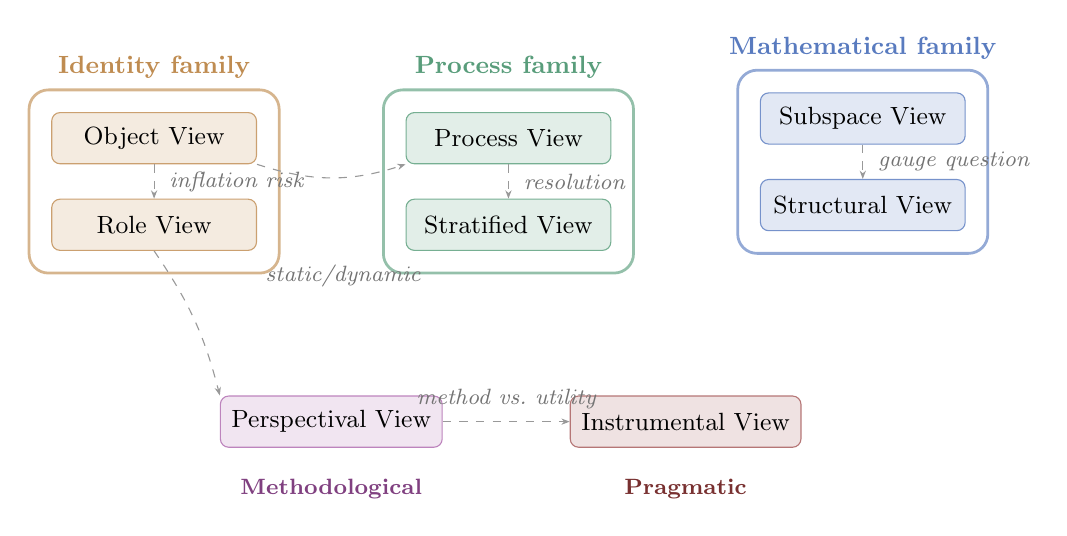
\begin{tikzpicture}[
  every node/.style={font=\small},
  bigbox/.style={draw, rounded corners=7pt, line width=1pt, inner sep=8pt},
  vn/.style={draw, rounded corners=3pt, minimum width=2.6cm,
             minimum height=0.65cm, align=center, inner sep=4pt},
  fl/.style={font=\small\bfseries, align=center},
  tl/.style={font=\footnotesize\itshape, text=black!55},
  ta/.style={dashed, -{Stealth[length=3pt]}, black!40, thin},
]
\node[vn, fill=identity_c!15, draw=identity_c!70] (obj) at (0,0)     {Object View};
\node[vn, fill=identity_c!15, draw=identity_c!70] (rol) at (0,-1.1)  {Role View};
\node[bigbox, identity_c!55, fit=(obj)(rol),
      label={[fl,text=identity_c!85]above:Identity family}] {};
\node[vn, fill=process_c!15, draw=process_c!70]   (pro)   at (4.5,0)    {Process View};
\node[vn, fill=process_c!15, draw=process_c!70]   (strat) at (4.5,-1.1) {Stratified View};
\node[bigbox, process_c!55, fit=(pro)(strat),
      label={[fl,text=process_c!85]above:Process family}] {};
\node[vn, fill=math_c!15, draw=math_c!70] (sub) at (9.0, 0.25)  {Subspace View};
\node[vn, fill=math_c!15, draw=math_c!70] (str) at (9.0,-0.85)  {Structural View};
\node[bigbox, math_c!55, fit=(sub)(str),
      label={[fl,text=math_c!85]above:Mathematical family}] {};
\node[vn, fill=persp_c!15, draw=persp_c!70] (per) at (2.25,-3.6) {Perspectival View};
\node[font=\footnotesize\bfseries, text=persp_c!80!black] at (2.25,-4.45) {Methodological};
\node[vn, fill=instru_c!15, draw=instru_c!70] (ins) at (6.75,-3.6) {Instrumental View};
\node[font=\footnotesize\bfseries, text=instru_c!80!black] at (6.75,-4.45) {Pragmatic};
\draw[ta] (obj.south) -- (rol.north) node[midway, right=2pt, tl] {inflation risk};
\draw[ta] (pro.south) -- (strat.north) node[midway, right=2pt, tl] {resolution};
\draw[ta] (sub.south) -- (str.north) node[midway, right=2pt, tl] {gauge question};
\draw[ta, bend right=18] (obj.south east) to (pro.south west);
\node[tl] at (2.4,-1.75) {static/dynamic};
\draw[ta, bend left=10] (rol.south) to (per.north west);
\draw[ta] (per.east) -- (ins.west) node[midway, above=1pt, tl] {method vs.\ utility};
\end{tikzpicture}
\caption{The eight views grouped into families by shared mathematical apparatus
  (identity, process, mathematical), with two singletons (methodological, pragmatic).
  Dashed arrows mark principal decision points and conflation risks discussed in
  Section~\ref{sec:decisions}.}
\label{fig:families}
\end{figure}

%% ---------------------------------------------------------------
\section{Relation to Companion Frameworks}\label{sec:companions}
%% ---------------------------------------------------------------

Three companion papers address complementary parts of the problem.  We
describe each and clarify what it presupposes and what it provides.

\paragraph{Mechanistic Validity \citep{tower2026mechval}.}
MechVal provides 27 criteria for evaluating whether a mechanistic
interpretability claim is warranted by evidence.  The criteria are
organized across five validity lenses (construct, internal, external,
measurement, interpretive) and a tier taxonomy (Speculative through
Established).

MechVal presupposes a claim type: it evaluates whether the evidence
supports the claim, not whether the claim is well-formed.  Mechanistic
Views is logically prior.  The MechVal lens for interpretive validity
includes a level-declaration criterion (V1) requiring every quantitative
claim to be labeled with its level of analysis.  Mechanistic Views
provides the vocabulary for those labels: an activation-patching result
is an object-level observation; a DAS result (subject to the Sutter
constraint) is a subspace-level observation; a holonomy measurement is
a structural-level invariant.

\paragraph{The Geometry of Mechanisms \citep{tower2026geom}.}
This paper provides the formal mathematical objects that the subspace
and structural views implicitly require: Grassmannian structural causal
models (G-SCMs), parallel transport maps between Grassmannians, holonomy
groups, and sheaf cohomology organized over the circuit graph.  The
G-SCM makes the subspace view precise: mechanisms are subspace-valued
causal variables, and evidence is organized into three functors
($\mathcal{E}_{\mathrm{struct}}$, $\mathcal{E}_{\mathrm{causal}}$,
$\mathcal{E}_{\mathrm{dynamic}}$).

The paper also develops a conjecture about the injectivity of joint
evidence:

\begin{conjecture}[Evidence injectivity; \citealt{tower2026geom}]\label{conj:injectivity}
Each of the three evidence functors $\mathcal{E}_{\mathrm{struct}}$,
$\mathcal{E}_{\mathrm{causal}}$, and $\mathcal{E}_{\mathrm{dynamic}}$
fails to identify mechanisms that the other two can distinguish.  The
joint evidence functor $\mathcal{E} = (\mathcal{E}_{\mathrm{struct}},
\mathcal{E}_{\mathrm{causal}}, \mathcal{E}_{\mathrm{dynamic}})$ is
injective on the space of natural transformer mechanisms.
\end{conjecture}

We state this as a conjecture rather than a theorem because the
companion paper is a working draft and the result requires verification.
The claim that single-method evidence is insufficient for mechanism
identity is motivated by Proposition~\ref{prop:incoherence} and the
Sutter result; the claim that joint evidence is sufficient is an
empirical conjecture about the space of transformer mechanisms.

\paragraph{Weight-Space Circuit Analysis \citep{tower2026weight}.}
This paper provides empirical grounding for the structural view via
analysis of 123 geometric features extracted from static weight matrices.
The features recover known circuits at 84--100\% edge F1 with zero
forward passes, achieving weight--activation IIA correlation $r = 0.982$
across 432 head--task pairs.

The weight-space results are the natural evidence for the structural
view: they are distribution-free, defined before any input is shown
to the model, and invariant to prompt distribution and sampling.
The composition score $\|W_{O,u} W_{K,v}\|_F$ provides a distribution-free
upper bound on information flow that is a structural claim inaccessible
to activation-based methods.

%% ---------------------------------------------------------------
\section{Implications and Open Questions}\label{sec:implications}
%% ---------------------------------------------------------------

\paragraph{Stating the view is a publication norm.}
The primary practical implication of this paper is that mechanistic
interpretability claims should state the view under which they are made.
This is not bureaucratic overhead---it is a precision requirement of
the same kind as reporting which distribution patching was run on.
Object-level claims should be labeled as such, with the relevant
distribution specified.  Role claims should specify the role operationally
and report the independent tests.  Subspace claims should report the
identity criterion (same projector? geodesic distance below what
threshold?) and the subspace stability.  Structural claims should report
which symmetries were tested.  Process claims should report the
temporal evidence.

\paragraph{Evidence-claim matching.}
Each measurement type has a range: the set of claim types it can support.
A measurement whose range does not include the target claim type cannot
support that claim, regardless of how strong the measurement is.
Activation patching is not in the range of structural claims.
Single-method IIA without alignment constraint is not in the range of
any claim.  DAS with linear alignment is in the range of
one-dimensional subspace claims.  Stating the view makes these
range requirements explicit and checkable.

\paragraph{Views as research programs.}
The object and role views primarily organize and classify existing
empirical practice.  The subspace, structural, and stratified views
generate positive research programs: each calls for methods, results,
and formalism that do not yet exist.  For the subspace view: systematic
DAS studies with stability tests across models and distributions.  For
the structural view: holonomy measurements, gauge-invariance checks,
and the development of the sheaf cohomology formalism.  For the
stratified view: dimensionality diagnostics and stratum-transition
tests.  The atlas is therefore not merely a taxonomy of current
practice; it is a map of what is missing.

\paragraph{Open questions.}
Several questions are raised by the framework and not resolved:
\begin{enumerate}[leftmargin=*]
\item \emph{Process identity.}  The identity criterion for the process
      view (same dynamical basin or trajectory type) is underspecified
      relative to the object, subspace, and structural criteria.
      Formalizing process identity is an open problem.
\item \emph{Cross-view translation.}  Under what conditions can an
      object-level result be promoted to a subspace-level or structural-level
      result?  What additional evidence is required?  A systematic account
      of inter-view inference is missing.
\item \emph{Completeness of the atlas.}  The eight views are identified
      by reading the literature, not derived from the five axes.  Whether
      there are important views not represented---a Marr-level-2 computational
      view, a representational-content view, a population-level statistical
      view---is an open question.
\item \emph{View selection.}  The framework is pluralist but does not
      say which view to adopt for a given question.  A principled account
      of view selection---given a target phenomenon $T$, which view(s)
      are appropriate?---would extend the framework substantially.
\end{enumerate}

%% ---------------------------------------------------------------
\section{Conclusion}
%% ---------------------------------------------------------------

Mechanistic interpretability is not only a search for circuits.  It is
a search for the right kind of object to call a mechanism.  The field
already uses multiple mechanistic views, typically implicitly, and making
those views explicit improves both the precision of claims and the
appropriateness of evidence.

The central contribution is definitional: a mechanistic view is a
five-component structure $(O, {\sim}, E, F, T)$, and every
mechanistic interpretability result assumes one, whether or not it is
stated.  Coherence between the components is not automatic, and incoherent
views generate systematically unsatisfiable evidential demands.

The atlas of eight views---object, role, subspace, structural, process,
stratified, perspectival, instrumental---covers the main options
currently in use.  Each view is appropriate for some questions and
inappropriate for others.  The goal is not to collapse this plurality
into a master ontology but to make view choice explicit, justifiable,
and revisable.  The induction head result remains the canonical
illustration of what convergence across views looks like: object, role,
and process views all point to the same entity, which is why the result
supports claims that single-view results cannot.

\section*{Acknowledgments}

The MechVal framework, the geometric formalism, and the
weight-space experiments are developed in companion working papers.
All errors are the author's own.

%% ---------------------------------------------------------------
\appendix
\section{Coherence Violations: A Diagnostic Checklist}
%% ---------------------------------------------------------------

The following patterns indicate a coherence violation in the view
underlying a claim.

\begin{enumerate}[leftmargin=*, label=(\arabic*)]

\item \textbf{Ontology--identity mismatch.}  The ontology declares
      mechanisms to be concrete components, but the identity criterion is
      functional (two different components can be the same mechanism).
      Resolution: adopt the role view, which has functional identity built
      in, or restate the claim as object-level and drop cross-model
      generalization.

\item \textbf{Evidence out of range.}  A structural or subspace claim
      is supported only by activation-patching evidence.  Resolution:
      identify the view that patching evidence actually supports (object
      view) and state the structural or subspace claim as a hypothesis
      requiring further evidence.

\item \textbf{Unrestricted alignment.}  A subspace claim is supported
      by DAS/IIA without specifying the alignment class or reporting
      subspace stability.  By the Sutter result \citep{sutter2025}, high
      IIA under unrestricted nonlinear alignment is consistent with any
      causal structure.  Resolution: restrict the alignment class to
      linear maps or transport-respecting maps and report the eigenvalue gap.

\item \textbf{Process claim from checkpoint evidence.}  A claim about
      how a mechanism formed or why a behavior emerged at a certain scale
      is supported only by final-checkpoint analysis.  Resolution: either
      restate as a static claim or obtain training-dynamics evidence.

\item \textbf{Object-to-role slide.}  A component is identified by
      ablation and immediately labeled with a role without an independent
      test of the role specification.  Resolution: operationalize the role
      prediction and test it on held-out constructions.

\end{enumerate}

%% ---------------------------------------------------------------
\section{Full Axis Assignments}\label{app:axes}
%% ---------------------------------------------------------------

Table~\ref{tab:full} repeats the five-axis assignments from
Table~\ref{tab:atlas} and adds the characteristic failure mode for each
view.

\begin{table}[ht]
\centering
\footnotesize
\setlength{\tabcolsep}{3pt}
\begin{tabular}{p{0.09\linewidth}p{0.13\linewidth}p{0.13\linewidth}p{0.14\linewidth}p{0.12\linewidth}p{0.12\linewidth}p{0.17\linewidth}}
\toprule
\textbf{View} & \textbf{Ontology}
  & \textbf{Identity} & \textbf{Evidence}
  & \textbf{Formalism} & \textbf{Target}
  & \textbf{Failure mode} \\
\midrule
Object
  & Concrete part
  & Component overlap
  & Ablation, patching
  & Directed graph
  & Specific behavior
  & Role inflation; distribution sensitivity \\[2pt]
Role
  & Functional role
  & Role equivalence
  & Role-specific causal tests
  & Functional decomp.
  & Functional class
  & Role proliferation; underdefined roles \\[2pt]
Subspace
  & Causal subspace
  & Same projector
  & DAS/IIA (linear)
  & $\Gr(k,d)$
  & Representational variable
  & Sutter vacuousness; SAE conflation \\[2pt]
Structural
  & Gauge-invariant structure
  & Gauge orbit
  & Holonomy, composition
  & Fiber bundle
  & Computation class
  & False gauge invariance; arch.\ prior confound \\[2pt]
Process
  & Formation trajectory
  & Trajectory type
  & Checkpoints, knockouts
  & Dynamical system
  & Mechanism origin
  & Process--circuit conflation; training overfitting \\[2pt]
Stratified
  & Stratum point
  & Stratum + local equiv.
  & Dimensionality, rank
  & Whitney strat.
  & Resolution-relative
  & Stratum misidentification from method artifacts \\[2pt]
Perspectival
  & Method projection
  & Cross-method coherence
  & Multi-method robustness
  & Measurement algebra
  & Method-relative
  & Anti-realist slide; perspectival conflation \\[2pt]
Instrumental
  & Predictive model
  & Predictive equiv.
  & Forecast, intervention
  & Model theory
  & Behavior prediction
  & Safety-relevant overreach \\
\bottomrule
\end{tabular}
\caption{Full axis assignments and characteristic failure modes.}
\label{tab:full}
\end{table}

%% ---------------------------------------------------------------
\bibliographystyle{plainnat}
\begin{thebibliography}{99}

\bibitem[Bricken et~al.(2023)]{bricken2023}
Trenton Bricken, Adly Templeton, Joshua Batson, Brian Chen, Adam Jermyn,
  Tom Conerly, Nicholas L.\ Turner, Cem Anil, Carson Denison, Amanda Askell,
  Robert Lasenby, Yifan Wu, Shauna Kravec, Nicholas Schiefer, Tim Maxwell,
  Nicholas Joseph, Zac Hatfield-Dodds, Alex Tamkin, Karina Nguyen, Brayden
  McLean, Josiah E.\ Burke, Tristan Hume, Shan Carter, Tom Henighan, and
  Chris Olah.
\newblock Towards monosemanticity: Decomposing language models with dictionary
  learning.
\newblock \emph{Transformer Circuits Thread}, 2023.
\newblock \url{https://transformer-circuits.pub/2023/monosemanticity}.

\bibitem[Craver(2007)]{craver2007}
Carl F.\ Craver.
\newblock \emph{Explaining the Brain: Mechanisms and the Mosaic Unity of
  Neuroscience}.
\newblock Oxford University Press, Oxford, 2007.

\bibitem[Elhage et~al.(2021)]{elhage2021}
Nelson Elhage, Neel Nanda, Catherine Olsson, Tom Henighan, Nicholas Joseph,
  Ben Mann, Amanda Askell, Yuntao Bai, Anna Chen, Tom Conerly, Nova DasSarma,
  Dawn Drain, Deep Ganguli, Zac Hatfield-Dodds, Danny Hernandez, Andy Jones,
  Jackson Kernion, Liane Lovitt, Kamal Ndousse, Dario Amodei, Tom Brown, Jack
  Clark, Jared Kaplan, Sam McCandlish, and Chris Olah.
\newblock A mathematical framework for transformer circuits.
\newblock \emph{Transformer Circuits Thread}, 2021.
\newblock \url{https://transformer-circuits.pub/2021/framework}.

\bibitem[Geiger et~al.(2021)]{geiger2021}
Atticus Geiger, Hanson Lu, Thomas Icard, and Christopher Potts.
\newblock Causal abstractions of neural networks.
\newblock In \emph{Advances in Neural Information Processing Systems
  (NeurIPS)}, 2021.

\bibitem[Geiger et~al.(2024)]{geiger2024}
Atticus Geiger, Zhengxuan Wu, Christopher Potts, Thomas Icard, and Noah D.\
  Goodman.
\newblock Finding alignments between interpretable causal variables and
  distributed neural representations.
\newblock In \emph{Conference on Causal Learning and Reasoning (CLeaR)}, 2024.

\bibitem[Machamer et~al.(2000)]{machamer2000}
Peter Machamer, Lindley Darden, and Carl F.\ Craver.
\newblock Thinking about mechanisms.
\newblock \emph{Philosophy of Science}, 67\penalty0 (1):\penalty0 1--25, 2000.

\bibitem[Massimi(2022)]{massimi2022}
Michela Massimi.
\newblock \emph{Perspectival Realism}.
\newblock Oxford University Press, Oxford, 2022.

\bibitem[Olsson et~al.(2022)]{olsson2022}
Catherine Olsson, Nelson Elhage, Neel Nanda, Nicholas Joseph, Nova DasSarma,
  Tom Henighan, Ben Mann, Amanda Askell, Yuntao Bai, Anna Chen, et~al.
\newblock In-context learning and induction heads.
\newblock \emph{Transformer Circuits Thread}, 2022.
\newblock \url{https://transformer-circuits.pub/2022/in-context-learning-and-induction-heads}.

\bibitem[Sutter et~al.(2025)]{sutter2025}
Denis Sutter, Julian Minder, Thomas Hofmann, and Tiago Pimentel.
\newblock The non-linear representation dilemma: Is causal abstraction enough
  for mechanistic interpretability?
\newblock In \emph{Advances in Neural Information Processing Systems
  (NeurIPS)}, 2025.

\bibitem[Templeton et~al.(2024)]{templeton2024}
Adly Templeton et~al.
\newblock Scaling monosemanticity: Extracting interpretable features from
  {Claude 3 Sonnet}.
\newblock \emph{Anthropic Transformer Circuits Thread}, 2024.
\newblock \url{https://transformer-circuits.pub/2024/scaling-monosemanticity}.

\bibitem[Tower(2026a)]{tower2026mechval}
Elliot Tower.
\newblock Mechanistic validity: A multi-discipline framework for evaluating
  mechanistic claims in neural networks.
\newblock Working paper, 2026.

\bibitem[Tower(2026b)]{tower2026geom}
Elliot Tower.
\newblock The geometry of mechanisms: {G}rassmannian structural causal models,
  sheaf cohomology, and the triangulation conjecture.
\newblock Working paper, 2026.

\bibitem[Tower(2026c)]{tower2026weight}
Elliot Tower.
\newblock Weight-space circuit analysis: Structural geometry as empirical arm
  of causal mechanism theory.
\newblock Working paper, 2026.

\bibitem[Wang et~al.(2022)]{wang2022}
Kevin Wang, Alexandre Variengien, Arthur Conmy, Buck Shlegeris, and Jacob
  Steinhardt.
\newblock Interpretability in the wild: A circuit for indirect object
  identification in {GPT-2 Small}.
\newblock arXiv:2211.00593, 2022.

\bibitem[Woodward(2003)]{woodward2003}
James Woodward.
\newblock \emph{Making Things Happen: A Theory of Causal Explanation}.
\newblock Oxford University Press, Oxford, 2003.

\end{thebibliography}

\end{document}
